\documentclass[11pt,a4paper]{article}

\usepackage[margin=0.82in]{geometry}
\usepackage{booktabs}
\usepackage{longtable}
\usepackage{array}
\usepackage[table]{xcolor}
\usepackage{enumitem}
\usepackage{tikz}
\usetikzlibrary{positioning,arrows.meta,shapes.geometric,fit,backgrounds,calc}
\usepackage{amsmath}
\usepackage{float}
\usepackage{caption}
\usepackage{fancyhdr}
\usepackage{lastpage}
\usepackage{underscore}
\usepackage[hidelinks]{hyperref}

\definecolor{navy}{HTML}{102A43}
\definecolor{blue}{HTML}{1D70A2}
\definecolor{cyan}{HTML}{2E86AB}
\definecolor{green}{HTML}{2A9D8F}
\definecolor{amber}{HTML}{F4A261}
\definecolor{red}{HTML}{D95D39}
\definecolor{ink}{HTML}{243B53}
\definecolor{muted}{HTML}{627D98}
\definecolor{paleBlue}{HTML}{EAF4FA}
\definecolor{paleGreen}{HTML}{EAF7F4}
\definecolor{paleAmber}{HTML}{FFF4E6}
\definecolor{grid}{HTML}{CAD8E3}

\newcommand{\stImpl}{\textcolor{green}{\textbf{IMPLEMENTED}}}
\newcommand{\stPartial}{\textcolor{amber!80!black}{\textbf{PARTIAL}}}
\newcommand{\stGap}{\textcolor{red}{\textbf{GAP}}}
\newcommand{\stBlocked}{\textcolor{red}{\textbf{BLOCKED}}}
\newcommand{\stConditional}{\textcolor{blue}{\textbf{CONDITIONAL}}}
\newcommand{\code}[1]{\texttt{\small #1}}
\newcommand{\gate}[1]{\textcolor{blue}{\textbf{#1}}}

\hypersetup{
  pdftitle={SuryaGrid AI - Main Plan Execution Roadmap},
  pdfauthor={SuryaGrid Project Team},
  pdfsubject={Four-level execution plan, timeline, workflow, gates, and acceptance criteria}
}

\sloppy
\setlength{\emergencystretch}{3em}
\setlength{\parindent}{0pt}
\setlength{\parskip}{5pt}
\setlist[itemize]{leftmargin=1.35em,itemsep=2pt,topsep=3pt}
\setlist[enumerate]{leftmargin=1.55em,itemsep=2pt,topsep=3pt}
\renewcommand{\arraystretch}{1.18}

\pagestyle{fancy}
\fancyhf{}
\fancyhead[L]{\small\bfseries\textcolor{navy}{SURYAGRID AI}}
\fancyhead[R]{\small\textcolor{muted}{MAIN PLAN EXECUTION ROADMAP}}
\fancyfoot[L]{\footnotesize\textcolor{muted}{Version 1.0 | 9 July 2026}}
\fancyfoot[R]{\footnotesize\textcolor{muted}{Page \thepage\ of \pageref{LastPage}}}
\renewcommand{\headrulewidth}{0.5pt}
\renewcommand{\footrulewidth}{0.4pt}

\tikzset{
  level/.style={rectangle, rounded corners=2pt, thick, minimum height=1.1cm,
                text width=12.8cm, align=left, font=\small},
  workflow/.style={rectangle, rounded corners=2pt, draw=blue, fill=paleBlue,
                   text width=2.25cm, minimum height=1.15cm, align=center, font=\scriptsize},
  decision/.style={diamond, aspect=2, draw=amber!80!black, fill=paleAmber,
                   align=center, font=\scriptsize, inner sep=1pt},
  flow/.style={-{Stealth[length=2.2mm]}, thick, draw=navy},
  dashedflow/.style={-{Stealth[length=2.2mm]}, thick, dashed, draw=muted}
}

\newenvironment{callout}[2][paleBlue]
  {\begin{quote}\color{ink}\noindent
   \textcolor{blue}{\rule{2.5pt}{12pt}}\hspace{6pt}
   \textbf{\textcolor{navy}{#2}}\par\smallskip}
  {\par\smallskip\textcolor{grid}{\rule{\linewidth}{0.4pt}}\end{quote}}

\begin{document}

% ------------------------------------------------------------------ %
\begin{titlepage}
\pagecolor{navy}
\color{white}
\vspace*{2.3cm}

{\large\bfseries\textcolor{cyan!35}{SURYAGRID AI}\par}
\vspace{0.45cm}
{\Huge\bfseries Main Plan\par}
\vspace{0.15cm}
{\Huge\bfseries Execution Roadmap\par}
\vspace{0.7cm}
{\Large\textcolor{paleBlue}{Four-Level Timeline and Detailed Workflow}\par}
\vspace{0.9cm}
\textcolor{cyan!55}{\rule{0.86\textwidth}{1.1pt}}
\vspace{0.7cm}

{\large
Solar data and APIs $\rightarrow$ forecasting and ML $\rightarrow$ per-station generation
$\rightarrow$ demand gap $\rightarrow$ deterministic reward/penalty policy
$\rightarrow$ safe RL research $\rightarrow$ controlled integration
\par}

\vfill
\begin{tabular}{@{}rl@{}}
\textbf{Prepared by:} & SuryaGrid Project Team\\[4pt]
\textbf{Date:} & 9 July 2026\\[4pt]
\textbf{Repository baseline:} & commit \code{5bed3cd}\\[4pt]
\textbf{Scope:} & complete handwritten main plan, not only substation DSM\\[4pt]
\textbf{Planning horizon:} & 22 weeks from approved kickoff\\
\end{tabular}

\vspace{1.1cm}
{\small\textcolor{paleBlue}{
Evidence sources: both handwritten plan images, current repository, test/build results,
model cards, README, and report evidence matrix. Unclear handwriting and unapproved monetary
notes are identified as assumptions, never converted into facts.
}\par}
\end{titlepage}
\nopagecolor
\color{ink}

\tableofcontents
\newpage

% ------------------------------------------------------------------ %
\section{Executive Direction}

\begin{callout}{What this plan corrects}
The project is not only the recently implemented substation/DSM workflow. The governing
handwritten main plan contains \textbf{four levels}: data/API, forecasting and intelligence,
policy/economics, and operational workflow. Current Phase 1 work is a strong foundation, but
live settlement, production RL, and plant control remain gated.
\end{callout}

\begin{figure}[H]
\centering
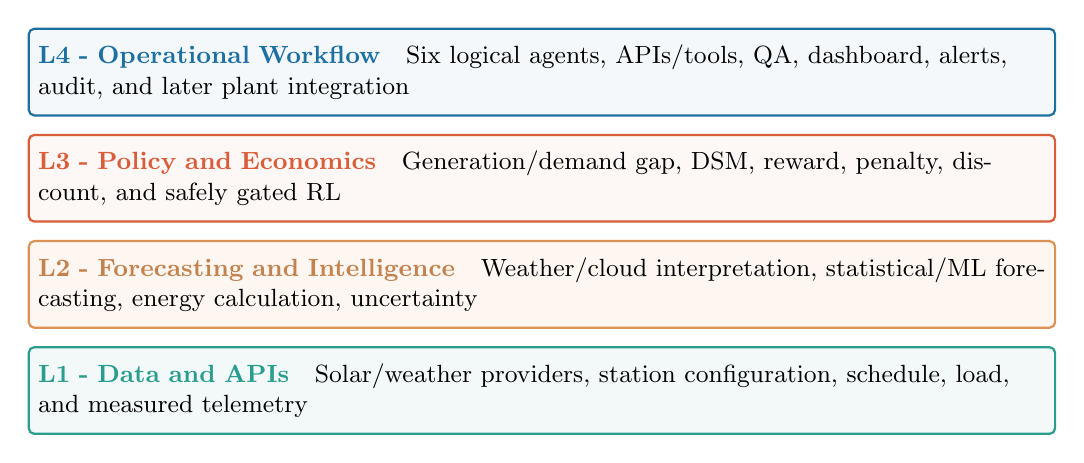
\begin{tikzpicture}[node distance=2.2mm]
\node[level, draw=blue, fill=blue!5] (l4)
  {\textbf{\textcolor{blue}{L4 - Operational Workflow}}\quad
   Six logical agents, APIs/tools, QA, dashboard, alerts, audit, and later plant integration};
\node[level, below=of l4, draw=red, fill=red!5] (l3)
  {\textbf{\textcolor{red}{L3 - Policy and Economics}}\quad
   Generation/demand gap, DSM, reward, penalty, discount, and safely gated RL};
\node[level, below=of l3, draw=amber!90!black, fill=amber!9] (l2)
  {\textbf{\textcolor{amber!80!black}{L2 - Forecasting and Intelligence}}\quad
   Weather/cloud interpretation, statistical/ML forecasting, energy calculation, uncertainty};
\node[level, below=of l2, draw=green, fill=green!6] (l1)
  {\textbf{\textcolor{green}{L1 - Data and APIs}}\quad
   Solar/weather providers, station configuration, schedule, load, and measured telemetry};
\end{tikzpicture}
\caption{The four-level main plan reconstructed from the handwritten source.}
\end{figure}

\begin{callout}[paleGreen]{Critical path}
Official rules and measured telemetry $\rightarrow$ reliable data foundation $\rightarrow$
site-level forecast validation $\rightarrow$ deterministic DSM/policy $\rightarrow$
secure operator workflow $\rightarrow$ shadow pilot.
\end{callout}

\begin{callout}[paleAmber]{Safety boundary}
Until official economics and measured outcomes exist, SuryaGrid is decision support.
No unsupported rupee settlement, no autonomous tariffs, and no plant dispatch. RL starts
offline and is advisory-only in shadow mode.
\end{callout}

\subsection{Reference delivery horizon}

For a cross-functional team of 3--5 engineers with part-time product, grid-domain, and
compliance support:

\begin{itemize}
  \item \textbf{Minimum credible decision-support pilot:} approximately 14--18 weeks.
  \item \textbf{RL-assisted, gated shadow pilot:} approximately 20--24 weeks.
  \item \textbf{External schedule risk:} official tariff, data, and pilot-site agreements can
        add 4--8 or more weeks.
\end{itemize}

% ------------------------------------------------------------------ %
\section{Source Interpretation and Scope Alignment}

\subsection{Governing sources}

\begin{enumerate}
  \item Main handwritten plan:
  \path{C:\Users\lekhan hr\Downloads\IMG_20260611_162613.jpg}.
  \item Handwritten Phase 1 note:
  \path{C:\Users\lekhan hr\Downloads\IMG-20260618-WA0001.jpg}.
  \item Verified repository state: \code{README.md},
  \code{docs/report/report_evidence_matrix.md}, code, tests, and model cards.
  \item Older \code{PROJECT_PLAN.md} and
  \code{SURYAGRID_PHASE1_ADVANCED_IMPLEMENTATION.md} are supporting interpretations only.
\end{enumerate}

\subsection{Main-plan intent}

\begin{longtable}{@{}p{1.0cm}p{4.1cm}p{9.4cm}@{}}
\caption{Main-plan level interpretation.}\label{tab:levels}\\
\toprule
\textbf{Level} & \textbf{Handwritten intent} & \textbf{Execution interpretation}\\
\midrule
\endfirsthead
\toprule
\textbf{Level} & \textbf{Handwritten intent} & \textbf{Execution interpretation}\\
\midrule
\endhead
\bottomrule
\endfoot
L1 & API / Solcast and data inputs &
Provider-neutral solar, weather, station, schedule, load, and telemetry foundation.\\
L2 & Cloud/weather, S/M, ML, station generation &
Data quality, solar/cloud/load forecasts, pvlib energy calculation, and uncertainty.\\
L3 & Cost, incentive, penalty, reward, discount, RL &
Approved deterministic policy first. RL only after real economics and measured telemetry.\\
L4 & Workflow &
Six logical agents, APIs/tools, QA, dashboard, alerts, audit, and later hardware/SCADA.\\
\end{longtable}

\subsection{Phase reconciliation}

The handwritten Phase 1 note asks for an irradiance nowcast, solar generation prediction,
agreement/scheduled-MW comparison, DSM threshold classification, penalty/no-penalty risk,
and a time-based generation/DSM timeline. The original Phase 1 specification implemented this
first as a toy-data/formula MVP. In the main plan's numbering, that work is closer to a
\textbf{simulation/foundation subset}, not the complete live pilot.

The repository now extends that baseline with real weather, pvlib, trained models, source
provenance, 344 substations, REST APIs, a Next.js interface, and deployment assets. For execution:

\begin{itemize}
  \item \textbf{Completed foundation:} historical toy/formula MVP plus current real-data prototype.
  \item \textbf{Current state:} decision-support prototype, not settlement of record or plant control.
  \item \textbf{Next release:} controlled live/shadow pilot for 1--3 sites.
  \item \textbf{Later release:} validated reward/discount policy, conditional RL, and read-only
        plant integration before any control consideration.
\end{itemize}

\subsection{Important interpretation cautions}

\begin{itemize}
  \item The main image explicitly marks L1, L2, L3, and L4. It is not a three-level-only plan.
  \item The unclear cloud role is named \textbf{Cloud/Weather Risk Agent}. The image does not
        reliably support the earlier ``Cloudinary Agent'' wording.
  \item S/M and one station-system acronym remain unresolved.
  \item Handwritten ``25'' and ``15\% discount'' notes are exploratory, not approved business rules.
  \item Solcast is an intended source, but its current integration is not verified.
\end{itemize}

% ------------------------------------------------------------------ %
\section{Verified Current Baseline}

The following checkpoint was verified on 9 July 2026. Backend tests and lint were run;
the frontend production build was run. No capability is upgraded based only on intended design.

\begin{footnotesize}
\begin{longtable}{@{}p{3.1cm}p{3.2cm}p{8.2cm}@{}}
\caption{Current implementation checkpoint.}\label{tab:baseline}\\
\toprule
\textbf{Capability} & \textbf{Status} & \textbf{Evidence and limitation}\\
\midrule
\endfirsthead
\toprule
\textbf{Capability} & \textbf{Status} & \textbf{Evidence and limitation}\\
\midrule
\endhead
\bottomrule
\endfoot
FastAPI backend and REST APIs & \stImpl & 61 \code{/api/v1} routes.\\
Automated verification & \stImpl & 118 backend tests passed; Ruff passed.\\
Next.js operator interface & \stImpl & Production build passed; 14 application routes.\\
Live weather & \stPartial & Open-Meteo operates; Solcast/NASA live failover is not wired.\\
Solar generation forecast & \stPartial & pvlib plus ML; output is estimated, not measured actual.\\
Cloud-risk forecast & \stImpl & Model cards and inference path exist.\\
Substation context & \stPartial & 344 OSM substations; capacity absent; voltage incomplete.\\
DSM classification & \stPartial & Decision-support framework; official monetary tariffs pending.\\
Reward/discount settlement & \stBlocked & Existing default amounts are illustrative and unapproved.\\
RL & \stBlocked & Research environment exists; production model card reports insufficient real data.\\
Authentication and tenancy & \stGap & Plans/settings exist; enforcement is incomplete.\\
SCADA/plant telemetry & \stGap & No verified connector or measured local PV/load.\\
Deployment & \stPartial & Docker/single-instance path exists; managed AWS is unverified code.\\
Production operations & \stGap & HTTPS, SLOs, monitoring, backup/restore need verification.\\
\end{longtable}
\end{footnotesize}

\subsection{Current truth boundaries}

\begin{itemize}
  \item PV generation is estimated from irradiance; it is not metered Bengaluru site truth.
  \item Substation capacity is missing for all 344 OSM records; dependent calculations must block.
  \item India-wide load and PV models remain non-production for local Bengaluru decisions.
  \item No real rupee DSM result is permitted until an approved, effective-dated rule source is
        parsed, independently reviewed, and tested.
  \item The RL policy is not production-ready and must remain blocked.
  \item Terraform proves intended architecture, not an actually deployed managed AWS stack.
\end{itemize}

% ------------------------------------------------------------------ %
\section{Target Operating Workflow}

\begin{figure}[H]
\centering
\resizebox{\textwidth}{!}{
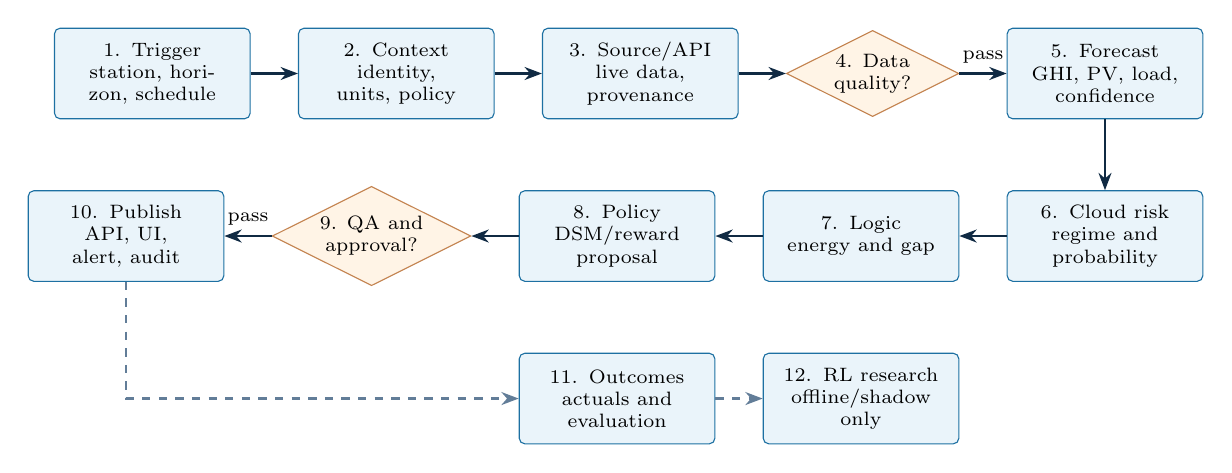
\begin{tikzpicture}[node distance=5mm and 6mm]
\node[workflow] (trigger) {1. Trigger\\station, horizon, schedule};
\node[workflow, right=of trigger] (context) {2. Context\\identity, units, policy};
\node[workflow, right=of context] (source) {3. Source/API\\live data, provenance};
\node[decision, right=of source] (dq) {4. Data\\quality?};
\node[workflow, right=of dq] (forecast) {5. Forecast\\GHI, PV, load, confidence};
\node[workflow, below=9mm of forecast] (cloud) {6. Cloud risk\\regime and probability};
\node[workflow, left=of cloud] (logic) {7. Logic\\energy and gap};
\node[workflow, left=of logic] (policy) {8. Policy\\DSM/reward proposal};
\node[decision, left=of policy] (qa) {9. QA and\\approval?};
\node[workflow, left=of qa] (publish) {10. Publish\\API, UI, alert, audit};
\node[workflow, below=9mm of policy] (actual) {11. Outcomes\\actuals and evaluation};
\node[workflow, right=of actual] (rl) {12. RL research\\offline/shadow only};

\draw[flow] (trigger) -- (context);
\draw[flow] (context) -- (source);
\draw[flow] (source) -- (dq);
\draw[flow] (dq) -- node[above,font=\scriptsize]{pass} (forecast);
\draw[flow] (forecast) -- (cloud);
\draw[flow] (cloud) -- (logic);
\draw[flow] (logic) -- (policy);
\draw[flow] (policy) -- (qa);
\draw[flow] (qa) -- node[above,font=\scriptsize]{pass} (publish);
\draw[dashedflow] (publish) |- (actual);
\draw[dashedflow] (actual) -- (rl);
\end{tikzpicture}}
\caption{Target end-to-end agent workflow. The dashed path records actual outcomes for
offline evaluation. Refetch and manual-review routes are specified in the detailed workflow.}
\end{figure}

\subsection{Detailed workflow}

\subsubsection*{A. Trigger and context}
\begin{enumerate}
  \item A scheduler or operator selects a station, horizon, schedule/request, and operating mode.
  \item The Orchestrator creates a trace ID and resolves station metadata, timezone, units,
        nameplate, permissions, and effective policy version.
  \item Missing required inputs are labelled and block dependent calculations.
\end{enumerate}

\subsubsection*{B. Data acquisition and quality}
\begin{enumerate}
  \setcounter{enumi}{3}
  \item The Source/API Agent retrieves live solar/weather data and recent measured actuals.
  \item Provider records are normalized to a canonical interval schema.
  \item Quality gates check freshness, completeness, range, units, timestamps, location,
        duplicates, source, and fallback state.
  \item Raw payloads and normalized records are stored with immutable lineage.
\end{enumerate}

\subsubsection*{C. Forecast and deterministic calculation}
\begin{enumerate}
  \setcounter{enumi}{7}
  \item The Forecast Agent produces irradiance, PV generation, and, when local data permits,
        load forecasts with confidence intervals.
  \item The Cloud/Weather Risk Agent produces cloud-regime and drop-risk probabilities.
  \item The Logic/Calculation Agent uses versioned pvlib and energy formulas to calculate
        interval energy, schedule-versus-expected gap, and constraints.
  \item When measured actual generation exists, forecast error and schedule deviation are
        calculated separately. A prediction is never labelled as measured actual.
\end{enumerate}

\subsubsection*{D. Policy, QA, and publication}
\begin{enumerate}
  \setcounter{enumi}{11}
  \item The Reward/Policy Agent applies the approved, effective-dated deterministic policy.
        Before approval, only risk/band output is allowed; rupee values remain disabled.
  \item Any policy or RL recommendation is bounded, explainable, advisory, and human-approved.
  \item QA checks source quality, model/formula version, bounds, confidence, policy version,
        and the complete calculation trace.
  \item Failed checks route to refetch, recompute, manual review, or a blocked state.
  \item Accepted results are persisted and exposed to the API, dashboard, timeline, alerts,
        reports, and audit log.
  \item Actual outcomes return later for monitoring and, only after the research gate, offline RL.
\end{enumerate}

% ------------------------------------------------------------------ %
\section{Six Logical Agent Contracts}

The repository can keep specialized modules, but product-level ownership should remain six
clear responsibilities that map to the main plan.

\begin{footnotesize}
\begin{longtable}{@{}p{2.5cm}p{3.1cm}p{3.4cm}p{3.1cm}p{2.6cm}@{}}
\caption{Logical agent contracts.}\label{tab:agents}\\
\toprule
\textbf{Agent} & \textbf{Input} & \textbf{Output} & \textbf{Failure behavior} &
\textbf{Initial release rule}\\
\midrule
\endfirsthead
\toprule
\textbf{Agent} & \textbf{Input} & \textbf{Output} & \textbf{Failure behavior} &
\textbf{Initial release rule}\\
\midrule
\endhead
\bottomrule
\endfoot
Orchestrator & station, horizon, schedule, mode & state, trace, final result &
bounded retry; honest block & no hidden agent decision\\
Source/API & provider config, coordinates, interval & normalized series and provenance &
failover or unavailable & two live providers before pilot\\
Forecast & quality-approved features & GHI/PV/load forecast and interval &
labelled formula fallback & site validation required\\
Cloud/Weather Risk & weather and irradiance features & cloud risk and confidence &
unknown-risk state & no invented camera input\\
Logic/Calculation & forecast, schedule, constraints & energy and gap calculations &
block missing dependencies & deterministic and versioned\\
Reward/Policy & gap, policy, approved economics & band or bounded proposal &
no-money blocked state & RL advisory only\\
\end{longtable}
\end{footnotesize}

% ------------------------------------------------------------------ %
\section{Execution Workstreams}

\subsection{A. Scope, policy, and evidence lock}
\textbf{When:} Weeks 0--1 \quad
\textbf{Owner:} Product lead + energy-domain lead + technical lead \quad
\textbf{Depends on:} none

\textbf{Tasks}
\begin{itemize}
  \item Approve the four-level scope and name each unclear handwritten concept.
  \item Select the first 1--3 pilot sites, personas, schedule source, settlement interval,
        and decision boundary.
  \item Disable or isolate unsupported monetary outputs.
  \item Freeze provenance labels, units, timezone rules, and missing-data behavior.
  \item Baseline APIs, model cards, tests, security gaps, and actual deployment topology.
\end{itemize}
\textbf{Exit gate:} signed scope/assumption register; no unapproved amount appears as regulatory
truth; pilot success metrics and blocked states are agreed.

\subsection{B. Official data and regulatory access}
\textbf{When:} Weeks 2--5; external lead time may add 4--8+ weeks \quad
\textbf{Owner:} Product/domain lead + data engineer \quad
\textbf{Depends on:} A

\textbf{Tasks}
\begin{itemize}
  \item Obtain applicable KERC/CERC/BESCOM DSM/tariff orders and legal review.
  \item Secure KPTCL/BESCOM/SLDC or pilot-site access to capacity, voltage, schedule, load,
        and interval actuals.
  \item Obtain plant nameplate, tilt/azimuth, inverter limits, meter definitions, interval,
        and timezone.
  \item Define licensing, consent, retention, sharing, and incident contacts.
  \item Write effective-dated source contracts and regulatory test cases.
\end{itemize}
\textbf{Exit gate:} approved regulatory source or explicit decision-support/no-money scope;
at least one pilot site supplies measured PV and schedule data; data ownership and quality
targets are recorded.

\subsection{C. L1 production data foundation}
\textbf{When:} Weeks 3--7 \quad
\textbf{Owner:} Backend/data team \quad
\textbf{Depends on:} A; overlaps B

\textbf{Tasks}
\begin{itemize}
  \item Add a second live provider; integrate Solcast if contractually required.
  \item Add provider health, persistent quotas, bounded retries, circuit breaking, and failover.
  \item Add immutable raw archive and idempotent normalized ingestion.
  \item Add late-data, duplicate, gap, range, timezone, unit, and quarantine controls.
  \item Operate backfill and live ingestion as observable jobs.
  \item Add time-series indexing/retention and source-to-feature lineage.
  \item Define station, schedule, actual-generation, load, and policy-version contracts.
\end{itemize}
\textbf{Exit gate:} 30 consecutive days of feed operation or approved accelerated window;
completeness at least 98\%; freshness target met; zero silent synthetic fallback; all outputs
resolve to source, timestamp, location, unit, and transformation.

\subsection{D. L2 forecast and calculation validation}
\textbf{When:} Weeks 6--11 \quad
\textbf{Owner:} ML/energy team \quad
\textbf{Depends on:} B for truth; C for ingestion

\textbf{Tasks}
\begin{itemize}
  \item Backtest irradiance and PV by site and season with time-based splits.
  \item Calibrate uncertainty and approve MAE/RMSE/bias/coverage thresholds.
  \item Validate cloud-risk output and its effect on confidence.
  \item Build local load forecasting only after local truth exists.
  \item Keep predicted generation, measured actual, schedule, and demand separate.
  \item Version pvlib assumptions, loss factors, inverter limits, and formulas.
  \item Add drift, missing-feature, bounds, champion/challenger, and rollback tests.
\end{itemize}
\textbf{Exit gate:} signed site-level model validation; uncertainty visible in API/UI;
labelled deterministic fallback or honest block, never fabricated actuals.

\subsection{E. L3 deterministic DSM and incentive policy}
\textbf{When:} Weeks 8--12 \quad
\textbf{Owner:} Domain lead + backend engineer + compliance reviewer \quad
\textbf{Depends on:} B and D

\textbf{Tasks}
\begin{itemize}
  \item Encode effective-dated rule profiles with regulator, region, denominator, interval,
        slabs, and source citation.
  \item Test boundaries, over/under generation, aggregation, and unit conversion.
  \item Separate forecasted DSM risk from settlement based on measured actuals.
  \item Define rewards and consumer discounts only after legal/business approval.
  \item Produce immutable calculation trace and manual recomputation worksheet.
  \item Require dual approval for rule publication and immediate rollback.
\end{itemize}
\textbf{Exit gate:} golden regulatory suite passes; independent recomputation matches;
unapproved profiles emit risk/band only and never currency.

\subsection{F. L4 secure operator workflow and integration}
\textbf{When:} Weeks 10--14 \quad
\textbf{Owner:} Frontend/backend/platform team \quad
\textbf{Depends on:} C; final acceptance uses D/E

\textbf{Tasks}
\begin{itemize}
  \item Implement JWT/OIDC, RBAC, tenant/site isolation, audit, and enforced rate limits.
  \item Make one station selection drive weather, solar, cloud, generation, DSM, source,
        and trace views.
  \item Show measured versus predicted state, missing data, confidence, and blocked reasons.
  \item Add alerts/reports with acknowledgment and escalation.
  \item Implement one read-only pilot connector using the site's approved interface.
  \item Keep all plant control commands disabled during the first pilot.
\end{itemize}
\textbf{Exit gate:} UAT passes normal, fallback, stale, missing, and blocked scenarios;
security tests prove isolation; connector replays data without controlling equipment.

\subsection{G. Safe RL research gate}
\textbf{When:} Weeks 12--17, conditional \quad
\textbf{Owner:} ML/research lead + domain reviewer \quad
\textbf{Depends on:} measured PV/load, approved economics, deterministic baseline

\textbf{Tasks}
\begin{itemize}
  \item Define state, action, constraints, reward, simulator, and forbidden actions.
  \item Train only on approved historical/simulated data with leakage checks.
  \item Compare against no-action and deterministic baselines.
  \item Stress-test rare weather, missing data, economic extremes, and policy changes.
  \item Expose recommendations only in shadow mode with bounds, reason, confidence, and rollback.
  \item Record proposal, human decision, outcome, and model/policy version.
\end{itemize}
\textbf{Exit gate:} offline policy improves agreed metrics with zero constraint violations;
domain/risk sign-off; RL remains advisory and cannot set tariffs, money, or dispatch.

If dependencies are absent at Week 12, pause this workstream without delaying the
decision-support pilot.

\subsection{H. Platform hardening and controlled pilot}
\textbf{When:} Hardening Weeks 14--18; pilot Weeks 19--22 \quad
\textbf{Owner:} Platform/SRE + QA + pilot owner \quad
\textbf{Depends on:} C--F; G only for RL-assisted pilot

\textbf{Tasks}
\begin{itemize}
  \item Verify HTTPS/domain, secrets, dependency scanning, CI/CD, and environment separation.
  \item Add logs, metrics, traces, data-quality alerts, drift alerts, and SLO dashboards.
  \item Test backup/restore, failover, provider outage, rollback, and incident response.
  \item Define and test availability, latency, and data-freshness targets.
  \item Run 2--4 weeks of shadow operation and compare forecasts with measured actuals.
  \item Hold production-readiness review and record accepted residual risk.
\end{itemize}
\textbf{Exit gate:} no critical security issue; restore and rollback drills pass;
pilot metrics and operator sign-off pass; go/extend/stop decision recorded.

% ------------------------------------------------------------------ %
\section{Integrated Timeline and Gates}

\begin{figure}[H]
\centering
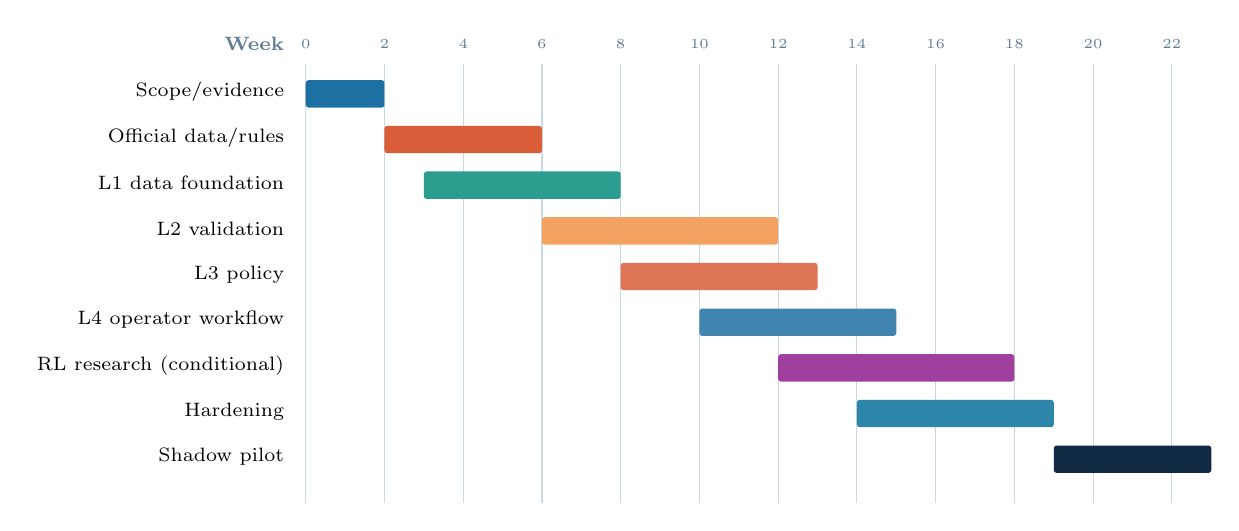
\begin{tikzpicture}[x=0.50cm,y=0.58cm]
  \def\xoff{5.1}
  \foreach \w in {0,2,...,22} {
    \draw[grid,thin] (\xoff+\w,0.2) -- (\xoff+\w,9.8);
    \node[font=\tiny,text=muted] at (\xoff+\w,10.25) {\w};
  }
  \node[font=\scriptsize\bfseries,text=muted,anchor=east] at (\xoff-0.3,10.25) {Week};

  \node[font=\scriptsize,anchor=east] at (\xoff-0.3,9.2) {Scope/evidence};
  \fill[blue,rounded corners=1pt] (\xoff+0,8.85) rectangle (\xoff+2,9.45);

  \node[font=\scriptsize,anchor=east] at (\xoff-0.3,8.2) {Official data/rules};
  \fill[red,rounded corners=1pt] (\xoff+2,7.85) rectangle (\xoff+6,8.45);

  \node[font=\scriptsize,anchor=east] at (\xoff-0.3,7.2) {L1 data foundation};
  \fill[green,rounded corners=1pt] (\xoff+3,6.85) rectangle (\xoff+8,7.45);

  \node[font=\scriptsize,anchor=east] at (\xoff-0.3,6.2) {L2 validation};
  \fill[amber,rounded corners=1pt] (\xoff+6,5.85) rectangle (\xoff+12,6.45);

  \node[font=\scriptsize,anchor=east] at (\xoff-0.3,5.2) {L3 policy};
  \fill[red!85,rounded corners=1pt] (\xoff+8,4.85) rectangle (\xoff+13,5.45);

  \node[font=\scriptsize,anchor=east] at (\xoff-0.3,4.2) {L4 operator workflow};
  \fill[blue!85,rounded corners=1pt] (\xoff+10,3.85) rectangle (\xoff+15,4.45);

  \node[font=\scriptsize,anchor=east] at (\xoff-0.3,3.2) {RL research (conditional)};
  \fill[violet!75,rounded corners=1pt] (\xoff+12,2.85) rectangle (\xoff+18,3.45);

  \node[font=\scriptsize,anchor=east] at (\xoff-0.3,2.2) {Hardening};
  \fill[cyan,rounded corners=1pt] (\xoff+14,1.85) rectangle (\xoff+19,2.45);

  \node[font=\scriptsize,anchor=east] at (\xoff-0.3,1.2) {Shadow pilot};
  \fill[navy,rounded corners=1pt] (\xoff+19,0.85) rectangle (\xoff+23,1.45);
\end{tikzpicture}
\caption{Dependency-based reference schedule. Week 0 is approved kickoff.}
\end{figure}

\begin{footnotesize}
\begin{longtable}{@{}p{1.5cm}p{5.0cm}p{5.2cm}p{2.7cm}@{}}
\caption{Integrated phase gates.}\label{tab:gates}\\
\toprule
\textbf{Week} & \textbf{Main work} & \textbf{Parallel work} & \textbf{Gate}\\
\midrule
\endfirsthead
\toprule
\textbf{Week} & \textbf{Main work} & \textbf{Parallel work} & \textbf{Gate}\\
\midrule
\endhead
\bottomrule
\endfoot
0--1 & Scope and evidence lock & Quarantine unsupported money & \gate{G0 Scope}\\
2--5 & Official rules and telemetry access & Provider/data contract design & \gate{G1 Source}\\
3--7 & L1 ingestion, quality, lineage & Security foundation & \gate{G2 Data}\\
6--11 & L2 site forecast validation & UI trace and provenance & \gate{G3 Model}\\
8--12 & L3 deterministic policy & Operator workflow & \gate{G4 Policy}\\
10--14 & L4 auth, UI, read-only connector & Alerts and UAT & \gate{G5 Pilot-ready}\\
12--17 & Conditional RL research & Hardening & \gate{G6 RL shadow}\\
14--18 & SRE/security hardening & Incident and restore drills & \gate{G7 Operations}\\
19--22 & Controlled 1--3-site shadow pilot & Drift and operator review & \gate{G8 Go/extend/stop}\\
\end{longtable}
\end{footnotesize}

\subsection{Dependency rules}

\begin{itemize}
  \item Frontend polish cannot compensate for missing source truth.
  \item Reward, discount, and currency cannot precede approved policy.
  \item RL cannot precede measured outcomes and a deterministic baseline.
  \item Control integration cannot precede read-only validation, security, audit, and human approval.
  \item A blocked dependency produces a smaller honest release; it does not permit fabricated data.
\end{itemize}

% ------------------------------------------------------------------ %
\section{Acceptance Scorecard}

\begin{longtable}{@{}p{2.8cm}p{11.7cm}@{}}
\caption{Pilot acceptance criteria.}\label{tab:acceptance}\\
\toprule
\textbf{Area} & \textbf{Required acceptance evidence}\\
\midrule
\endfirsthead
\toprule
\textbf{Area} & \textbf{Required acceptance evidence}\\
\midrule
\endhead
\bottomrule
\endfoot
Data & At least 98\% completeness in the agreed window; freshness SLO met;
100\% of outputs carry provenance.\\
Forecast & Site/season metrics meet signed thresholds; uncertainty is calibrated and visible.\\
Calculation & Golden energy/DSM cases are reproducible; units, formula, and policy version explicit.\\
Safety & No unsupported rupee output; no autonomous dispatch; missing inputs block honestly.\\
Security & Auth, RBAC, site isolation, rate limits, secrets, audit, and HTTPS are verified.\\
Reliability & Provider outage, retry, backup/restore, rollback, and stale-data tests pass.\\
Operator UX & User completes station-to-decision flow and understands confidence and limitations.\\
RL (optional) & Offline improvement over baseline with zero constraint violation;
advisory-only shadow mode.\\
\end{longtable}

% ------------------------------------------------------------------ %
\section{Risks and Responses}

\begin{footnotesize}
\begin{longtable}{@{}p{3.4cm}p{4.1cm}p{7.0cm}@{}}
\caption{Execution risks and planned responses.}\label{tab:risks}\\
\toprule
\textbf{Risk} & \textbf{Effect} & \textbf{Response}\\
\midrule
\endfirsthead
\toprule
\textbf{Risk} & \textbf{Effect} & \textbf{Response}\\
\midrule
\endhead
\bottomrule
\endfoot
Official rules delayed & No monetary settlement & Keep risk bands only; release decision support.\\
Measured PV/load unavailable & Forecast and RL cannot be locally validated &
Make pilot data agreement the top commercial task.\\
Solcast unavailable/costly & Source and quota risk &
Provider-neutral contract and second live fallback.\\
OSM station fields incomplete & Loading/voltage calculations blocked &
Obtain official capacity/voltage and preserve nulls.\\
India-model domain shift & Misleading local output &
Keep non-production and retrain on pilot-site truth.\\
Hard-coded money reaches UI & Regulatory and credibility harm &
Quarantine, label, and add tests forbidding unsupported currency.\\
RL optimizes unsafe proxy & Financial/operational harm &
Constrained actions, baselines, stress tests, shadow mode, and human approval.\\
Security stays aspirational & Cross-site data exposure &
Make enforcement and isolation tests a pilot gate.\\
Deployment differs from IaC claims & Reliability gap &
Verify actual topology and label code-only assets.\\
Ambiguous handwriting & Wrong product decomposition &
Maintain an assumption register and obtain owner confirmation.\\
\end{longtable}
\end{footnotesize}

% ------------------------------------------------------------------ %
\section{Deliverables}

\begin{enumerate}
  \item Approved scope and assumption register.
  \item Data-source, station, schedule, actual, load, and policy contracts.
  \item Reliable multi-provider ingestion with raw archive, quality gates, and lineage.
  \item Site-validated solar/load forecasts with model cards and uncertainty.
  \item Versioned deterministic energy and DSM library with golden tests.
  \item Secure operator dashboard, alerting, audit, and read-only connector.
  \item Operations package: CI/CD, observability, SLOs, backup/restore, rollback, incident runbook.
  \item Shadow-pilot report with data quality, accuracy, operator findings, and go/stop decision.
  \item Conditional RL evaluation report and advisory shadow policy.
\end{enumerate}

% ------------------------------------------------------------------ %
\section{Immediate Next 10 Working Days}

\begin{enumerate}
  \item Approve this roadmap and the permanent context prompt.
  \item Confirm the unclear cloud role, S/M term, regulator, settlement interval, and pilot boundary.
  \item Select 1--3 pilot sites and request nameplate, schedule, meter, PV actual, and load samples.
  \item Disable or isolate unsupported rupee outputs.
  \item Make one frontend station selection drive the full agent result and source trace.
  \item Verify hosted topology, HTTPS, production database content, and backup state.
  \item Draft provider/telemetry contracts and the official-rule evidence checklist.
  \item Open the regulatory/data-access workstream because it is the longest external dependency.
\end{enumerate}

% ------------------------------------------------------------------ %
\section{Permanent Context and Open Decisions}

The durable prompt is stored at:
\path{D:\Suryagrid AI\docs\SURYAGRID_MASTER_PLAN_CONTEXT_PROMPT.md}.
It records the main image interpretation, Phase 1 reconciliation, verified current baseline,
non-negotiable truth/safety rules, execution order, and future-agent response requirements.

Owner decisions still required:

\begin{itemize}
  \item Is Solcast mandatory, or is a provider-neutral source layer acceptable?
  \item Does the cloud role mean weather risk, cloud imagery/camera, or a media service?
  \item What do S/M and the unclear station-system acronym mean?
  \item Which Karnataka market participant and DSM regulation apply?
  \item What are the settlement interval, schedule source, and under/over-generation treatment?
  \item Which 1--3 sites can provide measured PV, schedule, load, and plant configuration?
  \item Is the first live release decision support only, or is any control action expected?
\end{itemize}

\begin{callout}[paleAmber]{Final accuracy note}
The two handwritten images are the primary intent sources, but parts of the main image are
illegible. ``Cloud/Weather Agent'' is a functional label, not a claim that the note says
``Cloudinary.'' The values 25 and 15\% are not approved requirements. All durations are planning
estimates and must be re-baselined after pilot data and regulatory access are confirmed.
\end{callout}

\end{document}
